\section{Support Programs for Initialization}
\label{Progs}

Links to all the programs mentioned here are under the ROMS web site:
\begin{verbatim}
      http://marine.rutgers.edu/po/models/roms.html
\end{verbatim}

\subsection{Grid generation}
\label{Grid}
On startup, SCRUM either reads a NetCDF file or calls \code{ana\_grid}
and \code{ana\_mask}
to find the location of the grid points, the grid metrics,
the bathymetry, the land/sea mask, and the
Coriolis parameter $f$.  If you won't be using \code{ana\_grid}, the
grid file must be generated before SCRUM can be run, either with
the programs in \code{gridpak} or with \code{SEAGRID}.

%\subsubsection{\code{ezgrid}}
%\label{Ez}
%\code{ezgrid} was written to generate a uniform rectangular grid
%with a simple bathymetry.  It has two modes, one for the upwelling
%example, and one for rectangular basins; the mode is determined by
%the \code{UPWELLING} switch in \code{cppdefs.h}.  If \code{UPWELLING}
%is not defined then the important parameters are:
%\begin{klist}
%   \kitem{xl}   basin length in the $\xi$-direction.
%   \kitem{el}   basin width in the $\eta$-direction.
%   \kitem{h0}   bottom depth.
%   \kitem{f0, beta}  Coriolis parameter with the $\beta$-plane
%   approximation, $f = f_o + \beta y$.
%\end{klist}
%In either case you will have to also set the name of the gridfile,
%\code{grdname}, near the top of the \code{ezgrid.F} file.
%Once these parameters are set to your chosen values, compile and run it:
%\begin{verbatim}
%        make ezgrid
%        ezgrid
%\end{verbatim}
%This should create a binary NetCDF file called \code{grdname}.

\subsubsection{\code{gridpak}}
SCRUM has been designed to be used with curvilinear orthogonal grids
for boundary-following domains, etc., so there are situations in which
you want a more flexible grid-generation program than \code{ezgrid}.
We have been working on a suite of programs called \code{gridpak},
including \code{xcoast}, an interactive boundary drawing program.
See above for instructions on obtaining \code{gridpak}
and its documentation.

\subsection{Masking}
\label{Mask}
\subsubsection{The \code{scrum\_mask} program}
SCRUM now supports the masking of land areas, for which it requires
some new input arrays.  These arrays are read from the grid NetCDF
file or computed in \code{ana\_mask}.
The mask is defined on $\rho$-points; see Fig.\ \ref{fmask} for an
example of a small domain with an
isolated island and a promontory adjacent to the boundary.
\begin{figure}[thb]
  \setlength{\unitlength}{0.0125in}%
  \begin{picture}(0,0)(-138,-18)%
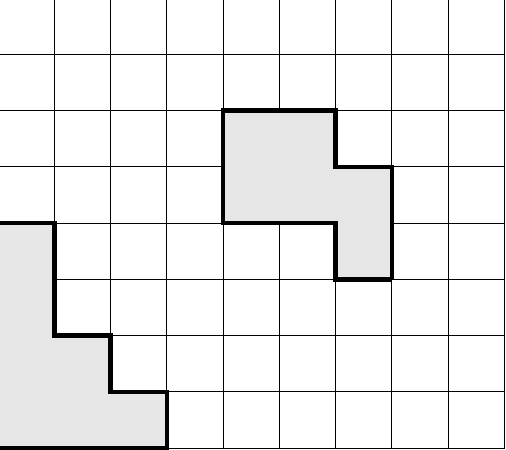
\includegraphics{pics/mask.pdf}%
  \end{picture}%
  \begin{picture}(300,264)(-9,461)
  \put(384,462){\makebox(0,0)[lb]{$i=\code{L}$}}
  \put(114,462){\makebox(0,0)[lb]{$i=1$}}
  \put( 93,477){\makebox(0,0)[lb]{$j=1$}}
  \put( 90,714){\makebox(0,0)[lb]{$j=\code{M}$}}
  \end{picture}
\caption{Small grid with masked regions}
\label{fmask}
\end{figure}
There are also arrays for the mask on $u$-points, $v$-points, and
$\psi$-points which are derived from the $\rho$-point mask.  The
$\psi$-point mask depends on the free-slip/no-slip option chosen
as described in \S\ref{Mask1}.

The programs in \code{gridpak} find the $\rho$-point mask based on the
bathymetry dataset.  Elevations at or above sea level are assumed to be
in the land mask.  You may choose to edit this mask, so Hernan Arango
has written a \code{Matlab} tool called \code{edit\_mask}.  It is an
interactive tool which requires \code{Matlab} as well as \code{mexnc}
for reading and writing NetCDF files from \code{Matlab}. On startup,
it will pop up file browsers, first for the grid file, then for a
coastline file. See Fig.\ \ref{fmat0} showing the file browser.

The view it presents is always rectangular, even for curvilinear grids,
but it will compute the coastline in the same (possibly) warped view to
allow a comparison. The first time you run it, it saves this mapped
coastline file to \code{ijcoast.mat} in the current directory.
Coastlines can be obtained from ...

\begin{figure}[pt]
  \setlength{\unitlength}{1 cm}%
  \begin{picture}(0,10)(0,0)%
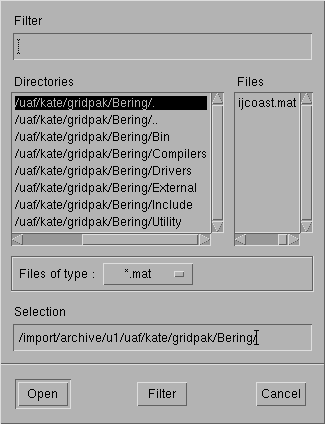
\includegraphics{pics/edit_mask0.png}
  \end{picture}
\caption{The \code{edit\_mask} file browser.}
\label{fmat0}
\end{figure}

An example of its use is shown in
Fig.\ \ref{fmat}, showing a Bering Sea grid.
It displays a rectangle for each $\rho$-point, including the
boundary ``image'' points.  The green/yellow boxes are land while the blue
ones are ocean. Figure \ref{fmat2} shows a zoomed in view where you
can actually see the individual boxes. Notice that scroll bars
appear automatically, allowing you to pan around.

Advice for masking details are as follows:
\begin{itemize}
  \item Make the ``image'' points have the same mask value as the points
they mirror. Something to avoid is an ocean image point adjacent
to a land point along an open boundary.
  \item Avoid one-grid bays such as the one that got away and is in
the right side of Fig.\ \ref{fmat2}. While these shouldn't cause the
model any direct grief, most plotting software cannot show you what
is happening in such places.
\end{itemize}

\begin{figure}[p]
  \setlength{\unitlength}{1 cm}%
  \begin{picture}(0,14)(0,0)%
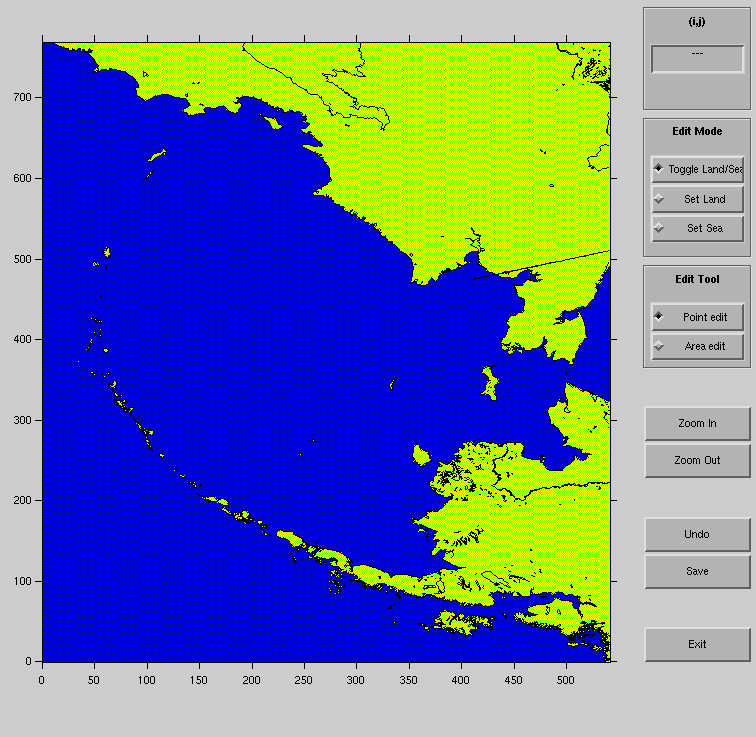
\includegraphics{pics/edit_mask1.png}
  \end{picture}
\caption{The \code{edit\_mask} program in action.}
\label{fmat}
\end{figure}

\begin{figure}[p]
  \setlength{\unitlength}{1 cm}%
  \begin{picture}(0,14)(0,0)%
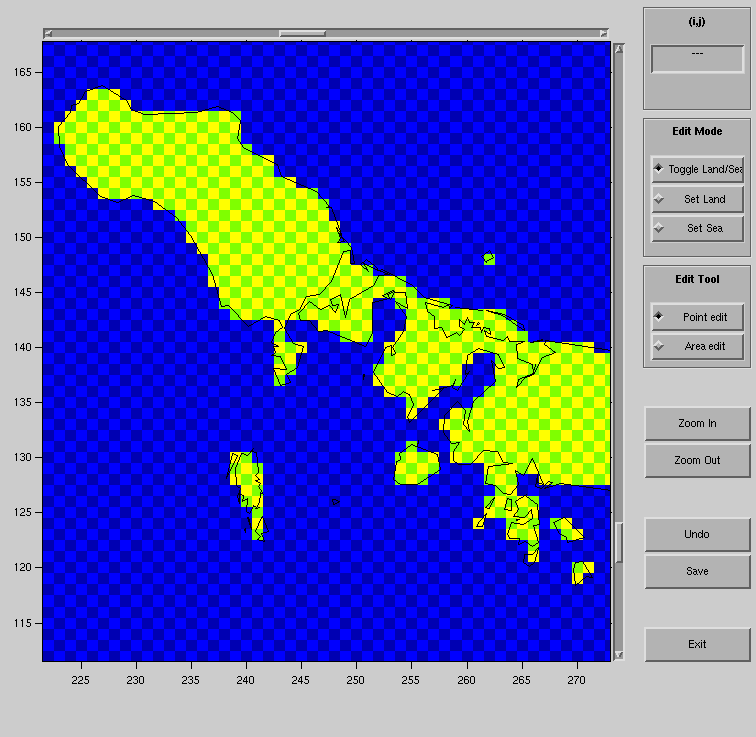
\includegraphics{pics/edit_mask2.png}
  \end{picture}
\caption{The \code{edit\_mask} program zoomed in.}
\label{fmat2}
\end{figure}

\subsection{Objective Analysis}
\label{OA}
[This section was contributed by Hernan Arango.]

The objective analysis (\code{oa}) package described here can be used
to prepare initial, climatology, update,  and forcing fields for SCRUM.
It maps oceanographic and atmospheric data to a specified application
grid.  Currently, it processes the following fields: {\sl in situ}
temperature, potential temperature, {\sl in situ} density anomaly,
salinity, sigma-t, sound speed, dynamic height, surface net heat flux
($Q$), surface freshwater flux, precipitation rate, evaporation rate,
incoming solar shortwave radiation, surface momentum (wind) stress
components, sea surface temperature (SST), and surface net heat flux
sensitivity to SST ($\partial Q / \partial {\rm SST}$).

This \code{oa} package is derived from an earlier program which Hernan
Arango and Carlos Lozano wrote at Harvard University in 1993.   The
basic algorithm used by this package is described in
\citet{Carter87}.  A comprehensive description of this
methodology can also be found in \citet{Gandin63,
Bretherton76, McWilliams86, Daley91, Bennett92}, and others.

Given observations $s_i = s({\bf x}_i, t_i)$ at location ${\bf x}_i,
t_i, i = 1, \ldots N$ an estimate $\phi_E$ of a scalar $\phi$ is
derived for location ${\bf x}$ and time $t$.  A linear unbiased estimate
is given by:
\[
   \phi_E({\bf x}, t) = \overline{\phi}({\bf x},t) + \sum_i w_i (s_i -
   \overline{s_i})
\]
for arbitrary $w_i$ since $\overline{\phi_E} = \overline{\phi}$.  The
associated variance of error is:
\[
  \overline{e^2(w)} = \overline{(\phi - \phi_E(w))^2}
\]
with $w = (w_1, \ldots w_N)$.  The overbar denotes an expected or
ensemble mean value.  The minimizer $w_*$:
\[
   \overline{e^2 (w_*)} \leq \overline{e^2(w)}
\]
is
\[
   w_* = {\bf A}^{-1} p
\]
with minimum error variance (Gauss-Markov):
\[
   \overline{e}^2_* = \overline{e^2(w_*)} = \overline{(\phi -
   \overline{\phi})^2} - p' {\bf A}^{-1} p
\]
Here, for convenience, matrix notation has been used.  $s = [s_1, \ldots
s_N]$ is a column correlation vector, $p = (\phi - \overline{\phi})(s
- \overline{s})$, and ${\bf A}$ is the covariance matrix:
\[
   {\bf A} = \overline{(s - \overline{s})(s - \overline{s})'}
\]
where the prime denotes a transpose.

Notice that ${\bf A}$ is symmetric.  In what follows, excluding
pathological cases, ${\bf A}$ is assumed to be positive definite.
The best linear estimate $\phi_*$ is then:
\[
   \phi_*({\bf x}, t) = \overline{\phi({\bf x}, t)} + p' {\bf A}^{-1}
   (s - \overline{s})
\]
with error $\overline{e^2_*}$.

The essential information required is statistical; namely the
spatial-temporal mean of the scalar and observations, the covariance
between observations, and the covariance between the scalar and the
observations.

The observations can be of different types, and different from the
scalar which you are trying to find.  Their usefulness is measured
by the fractional reduction of error:
\[
    {p'{\bf A}^{-1} p \over \overline{(\phi - \overline{\phi})^2}}
\]
In this package it is assumed that the covariance of the scalar is
homogeneous in space and homogeneous and isotropic in time:
\[
   C \left( ({\bf x_1}, t_1), ({\bf x_2}, t_2) \right) = 
   C \left( {\bf x_1 - x_2}, \left| t_2 - t_1 \right| \right)
\]
and errors at two different locations and times are uncorrelated:
\[
   E \left( ({\bf x}_1, t_1), ({\bf x}_2, t_2) \right) =
   E ({\bf x}_1, t_1) \delta ({\bf x_2 - x_1}) \delta(t_2 - t_1) .
\]
Currently, an analytical, isotropic, Gaussian correlation function is
assumed:
\[
    C({ \bf x_1 - x_2}, |t_2 - t_1| ) =
    {\cal C} ( |{ \bf x_1 - x_2}|, |t_2 - t_1| )
\]
with
\[
    {\cal C} ({\bf r}, \tau) = \exp \left[ - \left({\tau \over \tau_o}
    \right) ^2 \right] G({\bf r})
\]
\[
    G({\bf r}) = \left[ 1 - \left({{\bf r} \over a} \right)^2 \right]
    \exp \left[-\left({{\bf r} \over b} \right)^2 \right]
\]
where $\tau_o$ is the time decorrelation scale, $a$ is the zero
crossing distance, and $b$ is the spatial decorrelation scale.

This package uses a local solution to the \code{oa} equations.  That
is, only \code{nnce} influential observations are considered at each
mapped grid point.  This method is practical because it avoids
inverting large matrices when the number of observations is large.
Observations that are too far apart in space and time from the mapped
point contribute very little to the estimate, as one might expect.

\subsection{Forcing fields}
There are options for calling either \code{ana\_smflux} or
\code{get\_smflux} to get the surface momentum forcing.  If you do not
have an analytic formulation for this field,  you will have to create a
NetCDF forcing file which contains the surface momentum fluxes. This
file can be created with the \code{forcing} program, which reads the
output of the \code{oa} package.

The forcing file can
either contain one point value or a 2-D field of values.  Likewise, the
field can be constant in time or contain values for a series of times.
It is even possible to have a limited number of snapshots which get
cycled over in time.  For instance, you can provide 12 monthly mean
fields and tell it to cycle over these in a multi-year run.

The other forcing fields are treated in the same way and are also
contained in the NetCDF forcing file.  These include surface and bottom
heat and salt fluxes, the $\partial Q / \partial T$ and $T_{\rm ref}$
terms from \S\ref{vbc}, the incoming shortwave radiation used by the
Large et al.\ mixing scheme, and the wave information used by the
Styles and Glenn bottom boundary layer.  The ice thermodynamics also
requires forcing fields such as air temperature and cloud fraction.


\subsection{Initial and climatology fields}
The model will either read its initial fields from a NetCDF file or it
will compute them in \code{analytical.F}.  If it is not computing them,
the routine \code{get\_initial} will read a history file or a file
produced by the \code{initial} program.  This program in turn is
expecting to read the output of the \code{oa} program.

The model has the option of reading in 3-D climatology fields from a
climate NetCDF file.  This file contains the 3-D climatologies for the
tracers, perhaps at a number of times.  The subroutine \code{get\_clima}
will read this file and do any necessary time interpolations.  The
climate file is also produced by the \code{initial} program.  The
climatology could also be used for the boundary conditions, both for
the tracer values on inflow or for prescribed boundary conditions.  In
this case it would make more sense to only store the 2-D arrays.  We do
not yet have the software for handling these 2-D arrays, but it would
be a straightforward modification to the \code{initial} program.
